\documentclass[11pt]{article}
\usepackage[margin=1in]{geometry}
\usepackage{amsmath,amssymb,amsthm,bm}
\usepackage{booktabs,array}
\usepackage[most]{tcolorbox}
\usepackage{tikz}
\usetikzlibrary{arrows.meta,positioning,shapes.geometric,calc,fit,backgrounds}
\usepackage{listings}
\usepackage{float}
\usepackage{hyperref}
\usepackage{xcolor}
\usepackage{enumitem}
\hypersetup{colorlinks=true,linkcolor=blue!50!black,citecolor=blue!50!black,urlcolor=blue!50!black}

% ---- three-level boxes (house style, matching doc/algorithms_orbit_transfer.tex)
\newtcolorbox{eli}{colback=green!5,colframe=green!45!black,title=ELI5,fonttitle=\bfseries,breakable}
\newtcolorbox{intu}{colback=blue!4,colframe=blue!45!black,title=Intuition,fonttitle=\bfseries,breakable}
\newtcolorbox{rig}{colback=gray!6,colframe=black!70,title=Rigor,fonttitle=\bfseries,breakable}
\newtcolorbox{warn}{colback=orange!6,colframe=orange!70!black,title=Where it breaks / what is assumed,fonttitle=\bfseries,breakable}
\newtcolorbox{meas}{colback=purple!4,colframe=purple!50!black,title=Measured,fonttitle=\bfseries,breakable}

% ---- code snippets, sliced VERBATIM from the script at build time
\lstdefinestyle{mat}{language=Matlab,basicstyle=\ttfamily\scriptsize,keywordstyle=\color{blue!60!black},
  commentstyle=\color{green!40!black}\itshape,stringstyle=\color{purple!60!black},
  showstringspaces=false,breaklines=true,breakatwhitespace=false,columns=fullflexible,keepspaces=true,
  frame=single,rulecolor=\color{black!30},framesep=3pt,xleftmargin=2pt,aboveskip=4pt,belowskip=6pt}
\lstset{style=mat}
\newtcblisting{snippet}[1]{listing only,colback=white,colframe=black!40,title={\small\ttfamily\bfseries #1},
  fonttitle=\bfseries,breakable,listing options={style=mat},left=2pt,right=2pt,top=2pt,bottom=2pt}

\tikzset{
  box/.style={draw,rounded corners,align=center,minimum height=8mm,inner sep=4pt,fill=white},
  data/.style={draw,align=center,inner sep=4pt,fill=yellow!12,rounded corners=1pt,font=\small\ttfamily},
  gate/.style={draw,diamond,aspect=2.4,align=center,inner sep=1pt,fill=orange!10,font=\small},
  proc/.style={box,fill=blue!6},
  ext/.style={box,fill=green!8},
  outc/.style={box,fill=purple!8,font=\small},
  arr/.style={-{Latex[length=2mm]},thick},
  lbl/.style={font=\scriptsize,fill=white,inner sep=1pt}
}

\newcommand{\lv}{\lambda_v}\newcommand{\lr}{\lambda_r}\newcommand{\lm}{\lambda_m}
\newcommand{\tf}{t_f}\newcommand{\R}{\mathbb{R}}
\newcommand{\file}[1]{\texttt{#1}}
\newcommand{\sD}{s_D}\newcommand{\sA}{s_A}
\newcommand{\Tnd}{T_{\mathrm{nd}}}\newcommand{\cnd}{c_{\mathrm{nd}}}
\newcommand{\Tl}{\mathcal{T}}

\title{Where the First Root Comes From\\
\large A section-by-section guide to \file{root\_origins\_study.m}:\\
the cold lottery, the two-half ladder, the covector handoff, and the basin hunt}
\author{M.~Casey \quad (Coorbital, \file{orbit\_transfer/DRO\_tulip})}
\date{2026-09-16}

\begin{document}
\maketitle

\begin{abstract}
Every seed in the costate library is a previous root. So where did the first
one come from? \file{root\_origins\_study.m} answers that by doing it: it starts
from nothing but two periodic orbits and an engine, and measures the three
mechanisms that produce a first root --- a cold direct solve where the
problem is easy, a ladder down the engine axis that changes chart from
collocation to shooting halfway, and a branch-blind hunt for other families.
This guide walks the script section by section. Each section is explained
three times: as a picture (ELI5), as the reasoning needed to trust it
(Intuition), and as the equations and the code (Rigor), with the code
snippets sliced verbatim from the script at build time so they cannot drift
from it, and the campaign's measurements called out where they settled a
question. It ends with what the script does \emph{not} establish, because the
two external reviews of it (FINDINGS 76--77) were mostly about sentences that
claimed more than the computation earned. Companions:
\file{seeds\_and\_solution\_route.tex} (what a seed is),
\file{transfer\_study\_guide.tex} (the gate stack the certifier runs),
\file{process/ROOT\_ORIGINS\_STUDY.md} (how to run it).
\end{abstract}

\tableofcontents

%=========================================================================
\section{The question, and the honest answer first}
%=========================================================================

\begin{eli}
Imagine a library of maps for flying a small spacecraft from one orbit
around the Moon to another. Every map in the library was drawn by starting
from a neighbouring map and nudging it. Fine --- but somebody had to draw the
first map with no neighbour to copy. How?

For this particular library the honest answer is: the first map was a gift.
A converged transfer for exactly this cell arrived with the \file{pumpkynPie}
package, and every early measurement in the campaign is quoted against it.
This script is what you do for every other cell, thrust and orbit pair ---
which is nearly everything --- where there is no gift.
\end{eli}

\begin{intu}
Three mechanisms, in the order a campaign uses them, and each one is a
\emph{measurement} in the script rather than a claim:
\begin{enumerate}[nosep]
\item \textbf{The cold lottery} (Section~\ref{sec:lottery}). Solve the operating
      point cold, from nothing but the endpoints and a time-of-flight guess,
      at several mesh densities. The accepted solves do not agree. That
      motivates informed seeding or continuation rather than trusting one
      cold solve.
\item \textbf{The ladder} (Section~\ref{sec:direct}--\ref{sec:indirect}). Start
      where the problem is easy --- 15\,N, a half-day transfer under one
      turn, converges cold in seconds --- and walk the engine down, each rung
      seeded by the one above. The walk has two halves and a seam: direct
      collocation down to 0.5\,N, then a covector harvest, then multiple
      shooting the rest of the way.
\item \textbf{The basin hunt} (Section~\ref{sec:hunt}). From the root reached, ask
      the direct solver for other arrival phases. It is branch-blind: it lands
      wherever its warm start is near. That is a hazard if you assume it
      returns your family, and a discovery tool if you do not.
\end{enumerate}
\end{intu}

\begin{rig}
The problem throughout is the Earth--Moon CR3BP in rotating barycentric
nondimensional units ($\mu^\star=0.012150585609624$, $l^\star=389703.26$\,km,
$t^\star=382981.29$\,s), minimum time, low thrust, free $\tf$, fixed endpoints:
\[
\dot{\bm r}=\bm v,\qquad
\dot{\bm v}=\bm g(\bm r,\bm v)+\frac{\Tnd\,q}{m}\,\bm u,\quad \|\bm u\|=1,\ q\in[0,1],\qquad
\dot m=-\frac{\Tnd\,q}{\cnd},
\]
with $m$ a mass \emph{fraction} ($m(0)=1$), $\bm r(0),\bm v(0)$ on the DRO at
phase $\sD$ and $\bm r(\tf),\bm v(\tf)$ on the tulip at phase $\sA$. The
Hamiltonian, adjoints and the two facts the script leans on:
\[
H=1+\lr^{\!\top}\bm v+\lv^{\!\top}\bm g+\Tnd q\Big(\frac{\lv^{\!\top}\bm u}{m}-\frac{\lm}{\cnd}\Big),
\qquad
\bm u^\star=-\frac{\lv}{\|\lv\|},
\qquad
\dot\lm=-\frac{\partial H}{\partial m}=-\frac{\Tnd q\,\|\lv\|}{m^2}.
\]
\label{sec:q1}This is the normal, unconstrained minimum-principle formulation ($H=L+\lambda^{\!\top}\bm f$
with $L=1$, controls minimising $H$), with positive mass, no terminal-mass
penalty or active terminal-mass bound, and endpoint states that do not
depend on $\tf$. Under those assumptions the terminal mass is free, so
$\lm(\tf)=0$ (fixed terminal position and velocity do \emph{not} make
their costates vanish), and integrating backward,
\[
\lm(t)=\int_t^{\tf}\frac{\Tnd\,q(\xi)\,\|\lv(\xi)\|}{m(\xi)^2}\,\mathrm d\xi\ \ge\ 0 .
\]
After minimising over the direction, $\partial H/\partial q=-\Tnd\big(\|\lv\|/m+\lm/\cnd\big)$,
strictly negative wherever $\|\lv\|/m+\lm/\cnd>0$; minimising $H$ then
selects $q=1$. A nonzero primer is sufficient for that, not necessary.

\emph{Why primer zeros cannot spoil it.} The adjoints of $\bm r$ and $\bm v$
are linear and homogeneous in $(\lr,\lv)$:
$\dot\lr=-\bm g_r^{\!\top}\lv$, $\dot\lv=-\lr-\bm g_v^{\!\top}\lv$. At a
primer zero, $\dot\lv=-\lr$. If $\lr$ vanished there too, both would
vanish identically; then $\dot\lm=0$ and $\lm\equiv\lm(\tf)=0$, giving
$H\equiv1$, which contradicts $H(\tf)=0$. So primer zeros are isolated,
$q=1$ almost everywhere, and the direction's being undefined at isolated
instants does not change the trajectory: \textbf{minimum time is all-burn}
under these assumptions. An \emph{active} lunar-clearance constraint would
need the constrained minimum principle instead; the shooter uses the
unconstrained one.

The shooting unknown is $z=(\lambda(0),\tf)\in\R^8$, with $H(\tf)=0$
closing the free-time problem.
\end{rig}

%=========================================================================
\section{The flow of the script}
%=========================================================================

\emph{A note on numbering.} ``Script \S$n$'' and the \S$n$ in the section
headings and the diagram are the script's own section numbers, 0 to 8;
``Section~$n$'' is this document's. They differ by three.

\begin{intu}
Two things to notice in the diagram. The data objects change type at
script \S4: above it the trajectory is a discrete collocation solution
(\file{X}, \file{U}, and the NLP's multipliers); below it, it is a shooting
root ($z$ plus junction states). Script \S4 is the first place the
multipliers are \emph{mapped} into a state-and-costate shooting seed;
script \S7 harvests again, from each accepted probe. And the record
\file{S} grows as the run goes: the script checkpoints each completed mesh,
rung, handoff, certification and probe, so an hour-long run can be read
while it is still going. A stage interrupted mid-way may be absent, the
cold and direct records keep diagnostics rather than full solution arrays,
and a failed save warns rather than guaranteeing anything.
\end{intu}

\begin{figure}[!tbp]\centering
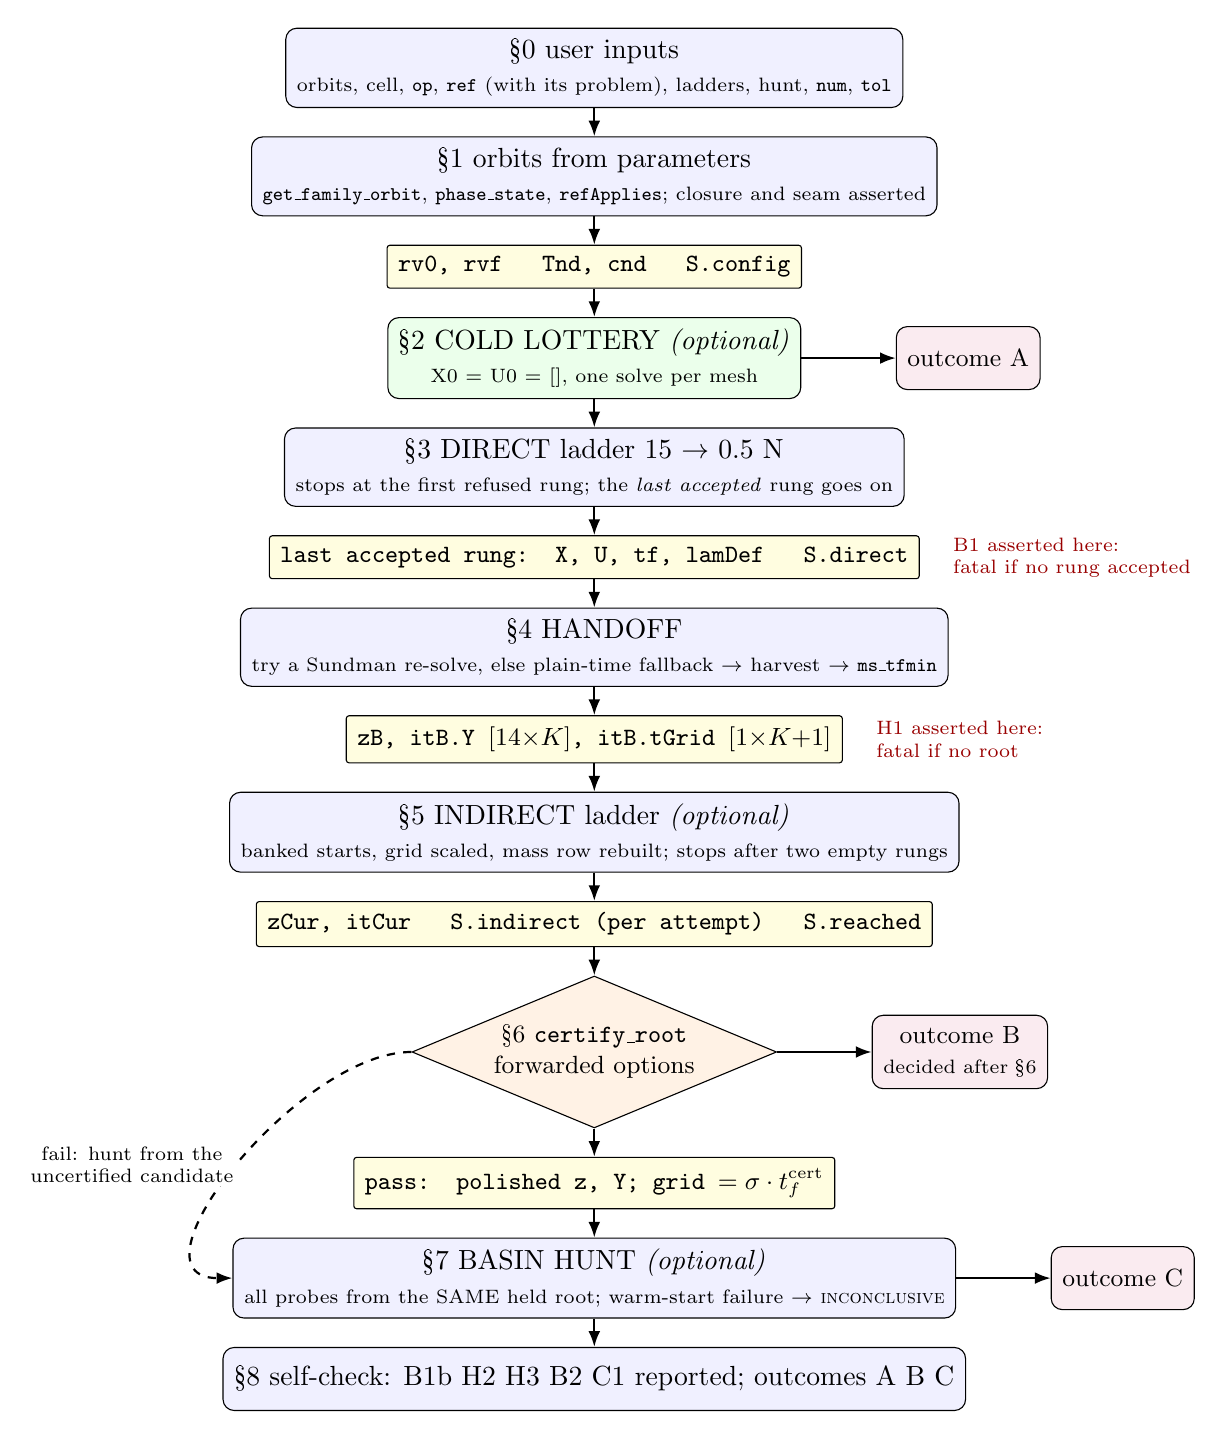
\begin{tikzpicture}[node distance=3.6mm]
\node[proc] (s0) {\S0 user inputs\\{\scriptsize orbits, cell, \file{op}, \file{ref} (with its problem), ladders, hunt, \file{num}, \file{tol}}};
\node[proc,below=of s0] (s1) {\S1 orbits from parameters\\{\scriptsize \file{get\_family\_orbit}, \file{phase\_state}, \file{refApplies}; closure and seam asserted}};
\node[data,below=of s1] (d1) {rv0, rvf \quad Tnd, cnd \quad S.config};
\node[ext,below=of d1] (s2) {\S2 COLD LOTTERY \emph{(optional)}\\{\scriptsize X0 = U0 = [], one solve per mesh}};
\node[proc,below=of s2] (s3) {\S3 DIRECT ladder 15 $\to$ 0.5 N\\{\scriptsize stops at the first refused rung; the \emph{last accepted} rung goes on}};
\node[data,below=of s3] (d3) {last accepted rung: X, U, tf, lamDef \quad S.direct};
\node[proc,below=of d3] (s4) {\S4 HANDOFF\\{\scriptsize try a Sundman re-solve, else plain-time fallback $\to$ harvest $\to$ \file{ms\_tfmin}}};
\node[data,below=of s4] (d4) {zB, itB.Y $[14{\times}K]$, itB.tGrid $[1{\times}K{+}1]$};
\node[proc,below=of d4] (s5) {\S5 INDIRECT ladder \emph{(optional)}\\{\scriptsize banked starts, grid scaled, mass row rebuilt; stops after two empty rungs}};
\node[data,below=of s5] (d5) {zCur, itCur \quad S.indirect (per attempt) \quad S.reached};
\node[gate,below=of d5,inner sep=2pt] (s6) {\S6 \file{certify\_root}\\forwarded options};
\node[data,below=of s6] (d6) {pass: polished z, Y; grid $=\sigma\cdot t_f^{\mathrm{cert}}$};
\node[proc,below=of d6] (s7) {\S7 BASIN HUNT \emph{(optional)}\\{\scriptsize all probes from the SAME held root; warm-start failure $\to$ \textsc{inconclusive}}};
\node[proc,below=of s7] (s8) {\S8 self-check: B1b H2 H3 B2 C1 reported; outcomes A B C};
\node[outc,right=12mm of s2] (oA) {outcome A};
\node[outc,right=12mm of s6] (oB) {outcome B\\{\scriptsize decided after \S6}};
\node[outc,right=12mm of s7] (oC) {outcome C};
\node[font=\scriptsize,text=red!60!black,align=left,right=3mm of d3] (f1) {B1 asserted here:\\fatal if no rung accepted};
\node[font=\scriptsize,text=red!60!black,align=left,right=3mm of d4] (f2) {H1 asserted here:\\fatal if no root};
\draw[arr] (s0)--(s1); \draw[arr] (s1)--(d1); \draw[arr] (d1)--(s2); \draw[arr] (s2)--(s3); \draw[arr] (s3)--(d3);
\draw[arr] (d3)--(s4); \draw[arr] (s4)--(d4); \draw[arr] (d4)--(s5); \draw[arr] (s5)--(d5);
\draw[arr] (d5)--(s6); \draw[arr] (s6)--(d6); \draw[arr] (d6)--(s7); \draw[arr] (s7)--(s8);
\draw[arr] (s2.east)--(oA); \draw[arr] (s6.east)--(oB); \draw[arr] (s7.east)--(oC);
\draw[arr,dashed] (s6.west) to[out=180,in=180] node[lbl,left,align=center]{fail: hunt from the\\uncertified candidate} (s7.west);
\end{tikzpicture}
\caption{Execution order, top to bottom; the \S{} numbers are the script's
own. Yellow boxes are the objects handed on. The two red notes are the
named fatal checks, asserted where their stage ends --- other validation
assertions (orbit closure, usable multipliers, a malformed passing
certificate) can also abort. Optional stages can be switched off in script
\S0; outcome B is decided only after certification, because ``reached the
target engine'' and ``holds a certified root there'' are different claims.}
\end{figure}

%=========================================================================
\section{\S0 --- User inputs and the units}\label{sec:inputs}
%=========================================================================

\begin{eli}
Everything the run depends on sits in one place at the top: which two
orbits, which point on each, what engine we are trying to reach, the two
ladders that get there, where to hunt, how long each step may take, and how
close is close enough. Change the experiment here and nowhere else.
\end{eli}

\begin{intu}
The reference deserves a word. The campaign's certified root at this cell
is stored with the \emph{problem it belongs to} --- orbits, phases, engine,
mass --- and reference comparisons are computed only when the live problem
matches. Otherwise the script says the reference belongs elsewhere; the cold
table keeps its ``vs ref'' column but shows NaN in it, and the summary and
the certified-root comparison suppress the number. Without that guard,
editing the cell would leave a figure on screen labelled ``the campaign's
answer here'' that belongs to somewhere else.
\end{intu}

\begin{snippet}{section 0: the operating point}
op = struct( ...
    'thrustN', 0.070, ...    % N   -- the abstract's Hall thruster
    'ispS',    900,   ...    % s
    'm0kg',    150);         % kg
\end{snippet}
\begin{snippet}{section 0: the reference carries its problem}
ref = struct('tfDays', 17.7976, 'tau', 1.0, 'Np', 7, 'pm', -1, 'sD', 0.0, 'sA', 0.0754, ...
             'thrustN', 0.070, 'ispS', 900, 'm0kg', 150, ...
             'what', 'the fast-family anchor of the 70 mN library (arrived with pumpkynPie)');
\end{snippet}

\begin{rig}
Nondimensionalisation. With $g_0=9.80665$\,m/s$^2$ and the CR3BP units,
\[
\Tnd=\frac{T}{m_0}\,\frac{t^{\star 2}}{1000\,l^\star},\qquad
\cnd=\frac{I_{sp}}{t^\star}\,g_{0,\mathrm{nd}},\qquad
g_{0,\mathrm{nd}}=g_0\,\frac{t^{\star 2}}{1000\,l^\star},
\]
so $\Tnd$ is the thrust acceleration at unit mass fraction and $\cnd$ the
exhaust speed, both in ND. The factor 1000 converts $l^\star$ from km to m.
The tolerance block keeps two kinds of number apart on purpose: what a
solver is \emph{asked} for (\file{Rsolve}, $10^{-11}$) and what a gate
\emph{accepts} ($R$, $10^{-8}$). A solve that plateaus above its own target
but inside the gate is a root.
\end{rig}

\begin{snippet}{section 0: the ND conversions}
g0  = 9.80665*tStar^2/(1000*lStar);
ndT = @(TN, m) (TN/m)*tStar^2/(lStar*1000);       % N -> ND thrust acceleration at m = 1
ndC = @(isp)   (isp/tStar)*g0;                    % s -> ND exhaust speed
\end{snippet}
\begin{snippet}{section 0: acceptance thresholds and solve targets}
tol = struct( ...
    'closure',   1e-7,  ...  % orbit periodicity
    'seamDeriv', 1e-6,  ...  % interpolant derivative mismatch across s = 0
    'defect',    1e-8,  ...  % collocation defect on an accepted rung
    'interp',    1e-8,  ...  % Hermite-Simpson interpolation residual (NOT in maxDefect)
    'tfSpread',  1e-8,  ...  % lifted-time continuity across the nodes
    'termErr',   1e-7,  ...  % terminal boundary residual
    'unit',      1e-8,  ...  % |u| = 1 on the solved directions
    'thrMin',    1e-3,  ...  % 1 - throttle: the throttle is FREE, so saturation is CHECKED (see above)
    'R',         1e-8,  ...  % multiple-shooting residual, inf-norm (acceptance)
    'Rsolve',    1e-11, ...  % what the shooting solver is ASKED for (tighter than the gate)
    'tfCluster', 0.02,  ...  % ND-relative spread within which two t_f are one cluster
    'same',      1e-2);      % |t_f - the reference's|/t_f to call the flight times equal
\end{snippet}

\begin{warn}
On \file{thrMin}: the direct solver leaves the throttle free \emph{by
design}, so that saturation can be checked rather than assumed. An
interior-point solver leaves a barrier slack on every bound --- measured
$4\times10^{-8}$ to $1.3\times10^{-6}$ at IPOPT tolerance $10^{-7}$, and the
first full run tripped a $10^{-6}$ gate on the 15\,N rung at $N=800$ with
$1.3\times10^{-6}$. A real switch takes the throttle to 0. The $10^{-3}$
gate sits between. It is a defensible \emph{seed-compatibility screen},
not a proof of saturation: its inequalities are strict, so it accepts a
sustained deficit just below 0.1\%, and a dip between the sampled stations
can escape it. The all-burn shoot and the certificate downstream are what
carry the claim.
\end{warn}

%=========================================================================
\section{\S1 --- The two orbits and the two endpoints}\label{sec:orbits}
%=========================================================================

\begin{eli}
Both orbits are rebuilt from their own parameters every run --- the DRO from
its period, the tulip from its petal count and branch --- and a point on each
is picked by a fraction of a period. No transfer is loaded anywhere; that is
the whole point of the script.
\end{eli}

\begin{intu}
Closure alone is not enough. An orbit can close to $10^{-7}$ and still have
an interpolant whose \emph{slope} jumps where phase wraps from $1$ back to
$0$. That matters here because phase is a continuation coordinate: nearby
phases seed related solves, and a kink at the wrap would make two
neighbouring endpoints disagree about the direction the orbit is moving.
So the smoothness across the seam is checked, not just the closure.
\end{intu}

\begin{rig}
\file{get\_family\_orbit} starts from a catalogued family seed and refines
it to closure; the script requires both sampled closures
$\|\bm x(T)-\bm x(0)\|<10^{-7}$. \file{phase\_state} returns a periodic
interpolant $s\mapsto\bm x(s)$ on $[0,1)$ with its seam diagnostics; the
script gates the larger seam-\emph{derivative} mismatch below $10^{-6}$
and does not separately gate the seam value. The endpoints are
$\bm x_0=\bm x_D(\sD)$, $\bm x_f=\bm x_A(\sA)$.
\end{rig}

\begin{snippet}{section 1: endpoints from phase fractions}
[stateD, seamD] = phase_state(tD, rvD);
[stateA, seamA] = phase_state(tT, rvT);
rv0 = stateD(phase.sD);   rv0 = rv0(1:6);
rvf = stateA(phase.sA);
\end{snippet}

%=========================================================================
\section{\S2 --- The cold lottery}\label{sec:lottery}
%=========================================================================

\begin{eli}
Ask the big optimiser to solve the real problem with no hints at all: just
the two endpoints, a guess at how long the trip takes, and how finely to
chop time. Do it three times, chopping time into 400, 800 and 1600 pieces.
Two of the three pass every acceptance check; the third stops at its
iteration limit. The two that pass give different trips, and nothing on
screen tells you which one you would have wanted.
\end{eli}

\begin{intu}
The direct method needs no previous converged transfer. With
\file{X0 = U0 = []} it still builds an initial numerical guess of its own ---
states linear between the endpoints, a mass ramp, thrust along the chord ---
and IPOPT takes it from there. Both things matter: whether it converges, and
\emph{what} it converges to. Minimum-time extremals of this problem come in
families, and a cold solve lands wherever its own discretisation happens to
lead. Only the mesh changes between the three runs; the answers change with
it. That motivates informed seeding or continuation on a catalog pair rather
than trusting one cold solve.

What the lottery does \emph{not} show, and the script now says so: that
each converged row is a distinct continuous extremal. Changing $N$ changes
the finite NLP, its internal guess and its conditioning; a flight-time
disagreement alone does not separate ``different physical extrema'' from
those effects. It is mesh sensitivity of the accepted \emph{discrete}
solutions --- which is enough for the point being made.
\end{intu}

\begin{rig}
The transcription is Hermite--Simpson with $N$ intervals on normalised time
$s\in[0,1]$, $h=1/N$. The flight time is \emph{lifted} to a per-node
variable $\Tl_j$ with continuity $\Tl_{k+1}=\Tl_k$, and the normalised-time
right-hand side is
\[
\bm F_j=\Tl_j\,\bm f(\bm x_j,\bm u_j,q_j),\qquad
\frac{\mathrm d\bm x}{\mathrm ds}=\tf\,\bm f .
\]
The defect and the midpoint interpolation are then
\begin{align*}
\bm x_{k+1}-\bm x_k-\frac{h}{6}\big(\bm F_k+4\bm F_{k+\frac12}+\bm F_{k+1}\big)&=0,\\
\bm x_{k+\frac12}-\frac{\bm x_k+\bm x_{k+1}}{2}-\frac{h}{8}\big(\bm F_k-\bm F_{k+1}\big)&=0,
\end{align*}
with $\Tl_{k+\frac12}=(\Tl_k+\Tl_{k+1})/2$; at feasibility every $\Tl_j=\tf$.
Equivalently, Hermite--Simpson applied to the augmented state $(\bm x,\Tl)$
with derivative $(\Tl\bm f,\,0)$. Lifting keeps each stencil local --- the
nodes, the midpoint and the local $\Tl$ of one interval --- so the KKT matrix
stays banded; a single scalar $\tf$ would add a dense bordering column (the
solver's own header records MATLAB dying on exactly that at $N=400$, an
implementation observation rather than a mathematical consequence). The
objective is $\tf$; the throttle is a free variable in $[0,1]$.

Every cold solve is judged by the same \emph{core} predicate as every other
direct solve in the script (\file{directOK}, Section~\ref{sec:direct}); a run that hit its
iteration limit is printed as an \emph{iterate} and excluded. On the
accepted rows the script reports the spread and a cluster count:
\[
n_{\mathrm{cluster}}=\big|\mathrm{uniquetol}\big(\{\tf^{(i)}\},\ \epsilon\big)\big|,\qquad
\epsilon=\texttt{tol.tfCluster}\times\min_i \tf^{(i)},\ \text{absolute},
\]
an explicit absolute tolerance tied to the shortest accepted flight time
(\file{uniquetol}'s default scales by the largest element, so a long outlier
would regroup the others). A cluster of flight times is not a basin --- two
roots can share a $\tf$ and one family can span several --- it is the cheap
first read of the table.
\end{rig}

\begin{snippet}{section 2: a genuinely cold solve}
oM = solveDirect(rv0, rvf, TndOp, cndOp, muStar, N, [], [], cold.tf0, dCold);
[okM, whyM] = directOK(oM, tol);
\end{snippet}
\begin{snippet}{section 2: the statistics on the accepted rows}
spread   = (max([good.tf]) - min([good.tf]))/min([good.tf]);
nCluster = numel(uniquetol([good.tf], tol.tfCluster*min([good.tf]), 'DataScale', 1));
below    = nnz([good.nodeRadiusKm] < num.clearKm);
agree    = nnz(abs([good.rel]) < tol.same);           % 0 when the reference does not apply
\end{snippet}

\begin{meas}
Reference at this cell: $\tf=4.0152$\,ND $=17.798$\,d. Cold, unconstrained,
same solver, same $\tf$ guess ($4.0$\,ND), only $N$ varying.

\begin{center}\small
\begin{tabular}{@{}rrrrl@{}}
\toprule
$N$ & $\tf$ (ND) & vs.\ reference & min node radius (km) & status \\
\midrule
\multicolumn{5}{@{}l@{}}{\emph{2026-08-03 (logged as altitude; $+1737.4$ here)}}\\
400  & 4.3807 & $+9.1\%$  & 6556 & converged \\
800  & 4.4507 & $+10.8\%$ & 1394 & converged, \textbf{through the Moon} \\
1600 & 4.7833 & $+19.1\%$ & 6417 & converged, 7.8\,m worst-interval error \\
\midrule
\multicolumn{5}{@{}l@{}}{\emph{2026-09-16, this script}}\\
400  & 4.6809 & $+16.6\%$ & 6563 & converged \\
800  & 4.9909 & $+24.3\%$ & 2243 & \emph{iterate}: iteration limit, excluded \\
1600 & 6.4126 & $+59.7\%$ & 1995 & converged \\
\bottomrule
\end{tabular}
\end{center}
Spread 37\%, two clusters, none within 1\% of the reference. Outcome A:
\textsc{supported}. ``Min node radius'' is over the collocation nodes ---
a screen, not a certified periselene.
\end{meas}

%=========================================================================
\section{\S3 --- The direct ladder}\label{sec:direct}
%=========================================================================

\begin{eli}
Start with an engine so strong the trip takes half a day and under one turn
around the Moon --- the optimiser finds that one cold in seconds. Then turn
the engine down a little, hand the optimiser the last trip as its starting
point, and solve again. Repeat. A good starting point usually makes each
solve easy; it does not guarantee the optimiser stays on the same family,
which is why every step is checked.
\end{eli}

\begin{intu}
Three things make the ladder work, and the script measures all three.

\emph{The next guess.} Between rungs the flight-time guess is scaled by
$\tf\leftarrow\tf\,(T_{\mathrm{prev}}/T)^{0.6}$, an empirical law for this
band. On the default run it predicts the next answer to about 1\% on most
rungs; the largest printed error is 2.1\%, on the last step,
$0.75\to0.5$\,N (guess $0.7416$\,ND, answer $0.7575$\,ND). The script prints
the ratio on every rung, so ``starts next to its answer'' is a number.

\emph{The screen.} A rung that lands far from where the scaling predicted
has landed somewhere the guess did not describe --- and it can look perfect
while doing so: converged, defect $10^{-14}$, clear of the Moon. Comparing
the answer with the guess that produced it is the only cheap thing that
catches it. It is a plausibility heuristic, not a branch detector: a sharp
turn on the same branch can trip it, and a jump to a nearby-time branch can
pass it. It applies to steps only, never to the cold top rung, whose guess
has no branch behind it (the true 15\,N answer is $41\times$ below the
$4.0$\,ND cold guess).

\emph{The throttle.} The solver leaves it free; every rung is checked to
have saturated, on both sides of 1, over the node and midpoint throttle
histories the solver returns (normally both; the predicate does not
separately require both arrays). Minimum time is all-burn, and a rung whose
throttle dipped would not be the problem the shooting solver solves next.
\end{intu}

\begin{snippet}{section 3: the inter-rung guess}
if ~isempty(Tprev), seedTf = seedTf*(Tprev/TN)^dladder.tfExp; end
\end{snippet}
\begin{snippet}{section 3: the band screen, steps only}
band = oR.tf/seedTf;
inBand = isempty(Tprev) || (band <= dladder.tfBand && band >= 1/dladder.tfBand);
clearR = radR >= num.clearKm;
okR = feasR && clearR && inBand;
\end{snippet}

\begin{rig}
\textbf{Delta-V falls down the ladder, and why.} At fixed exhaust speed
and initial mass the all-burn mass law is $m(t)=1-\Tnd t/\cnd$, so with
$a=\Tnd\tf/\cnd$ the propellant fraction used is $a$ and the ideal
\[
\Delta V_{\mathrm{nd}}=\cnd\ln\frac1{m_f}=-\cnd\ln(1-a),\qquad
\frac{\mathrm d\Delta V_{\mathrm{nd}}}{\mathrm da}=\frac{\cnd}{1-a}>0\quad(0\le a<1).
\]
If $\tf\propto T^{-0.6}$ then $T\,\tf\propto T^{0.4}$ \emph{falls} as
thrust falls, so $a$ falls and so do both the propellant and the ideal
$\Delta V$: lower thrust, longer trip, less propellant. The script prints the
dimensional value $\Delta V_{\mathrm{nd}}\,l^\star/t^\star$ in km/s.
Measured 15 $\to$ 0.5\,N: 4.22 $\to$ 0.996\,km/s, mass used 22.3\% $\to$
5.8\%.

\textbf{The predicate.} Every direct solve --- cold, ladder, Sundman
re-solve, hunt --- goes through one \emph{core} predicate, and each stage may
add its own screens on top (the ladder adds the lunar floor and the band;
the hunt adds the floor; the default lottery is unconstrained). Required
diagnostics default to NaN, not 0, so a missing one fails; the state array
must be finite; the throttle history must be finite and satisfy the strict
inequalities $1-\epsilon<q<1+\epsilon$. The first failed check is named, and
the reasons are reported in an order that never calls an unconverged
iterate a branch change.
\end{rig}

\begin{snippet}{section 3: ideal delta-V from the mass actually used}
dv = cnd*log(1/oR.mf)*lStar/tStar;               % ideal dV from the mass actually used
\end{snippet}
\begin{snippet}{local function directOK: one predicate for every direct solve}
fin = @(v) isnumeric(v) && isscalar(v) && isfinite(v) && isreal(v);
thrAll = [];
if isfield(o, 'U')  && ~isempty(o.U)  && size(o.U, 1)  >= 4, thrAll = [thrAll, o.U(4, :)];  end
if isfield(o, 'Um') && ~isempty(o.Um) && size(o.Um, 1) >= 4, thrAll = [thrAll, o.Um(4, :)]; end
thrLo = NaN;  thrHi = NaN;
if ~isempty(thrAll) && all(isfinite(thrAll)), thrLo = min(thrAll);  thrHi = max(thrAll); end
checks = { ...
  'not converged',          ~(isfield(o, 'success') && isscalar(o.success) && o.success); ...
  'non-finite fields',      ~(fin(gvd(o, 'tf', NaN)) && fin(gvd(o, 'mf', NaN)) && fin(gvd(o, 'maxDefect', NaN)) && ...
                              fin(gvd(o, 'termErr', NaN)) && fin(gvd(o, 'maxUnit', NaN))); ...
  'states not finite',      ~(isfield(o, 'X') && ~isempty(o.X) && all(isfinite(o.X(:)))); ...
  'collocation defect',     ~(gvd(o, 'maxDefect', NaN) < tol.defect); ...
  'interpolation residual', ~(fin(gvd(o, 'maxInterp', NaN)) && gvd(o, 'maxInterp', NaN) < tol.interp); ...
  'lifted t_f spread',      ~(fin(gvd(o, 'tfSpread', NaN)) && gvd(o, 'tfSpread', NaN) < tol.tfSpread); ...
  'terminal residual',      ~(gvd(o, 'termErr', NaN) < tol.termErr); ...
  '|u| = 1',                ~(gvd(o, 'maxUnit', NaN) < tol.unit); ...
  'throttle history',       ~(isfinite(thrLo) && isfinite(thrHi)); ...
  'throttle not saturated', ~(1 - thrLo < tol.thrMin); ...
  'throttle above one',     ~(thrHi - 1 < tol.thrMin); ...
  'mass fraction',          ~(gvd(o, 'mf', NaN) > 0 && gvd(o, 'mf', NaN) <= 1); ...
  't_f not positive',       ~(gvd(o, 'tf', NaN) > 0)};
bad = find([checks{:, 2}], 1);
ok = isempty(bad);
if ok, why = ''; else, why = checks{bad, 1}; end
\end{snippet}

\begin{meas}
Rung ratios matter. The first version of the ladder stepped $[15,10,5,2,1,0.5]$.
The $1\to0.5$\,N step (ratio 0.5) returned a converged solution with defect
$3.9\times10^{-14}$, a node clearance above the floor and $\|\bm u\|=1$ at $\tf=54.7$\,d and
$\Delta V=46.8$\,km/s: $16\times$ its own guess, 94\% of the mass burned, a
very different angular excursion. The ladder accepted it, and the handoff
then ground on a 54-day arc with integrator failures. The shipped rung set
steps by about 0.75 and does not jump; the band screen refuses the $16\times$
step. On the default run all eleven rungs accept, the worst throttle slack
is $1.3\times10^{-6}$, and $\tf$ goes $0.432\to3.358$\,d.
\end{meas}

%=========================================================================
\section{\S4 --- The handoff: where costates come from}\label{sec:handoff}
%=========================================================================

\begin{eli}
The big optimiser never heard of costates. But to enforce ``the trajectory
obeys physics'' at every step it keeps a set of bookkeeping numbers --- how
much the trip time would improve if it were allowed to cheat at that step.
Those bookkeeping numbers contain approximations to the steering costates.
After applying the right sign, scale and time-station mapping, lay them
along the trip at 25 checkpoints and hand that to the careful solver: it
now has a starting trajectory with the steering numbers filled in.
\end{eli}

\begin{intu}
Three subtleties turn that from a slogan into working code, and the script
checks two of them and says plainly that it cannot check the third.
\emph{Station}: in this transcription's covector mapping the defect
multipliers are associated with segment \emph{midpoints}; associating them
with nodes misplaces every harvested costate sample by half an interval,
which degrades the seed and biases any direct-versus-indirect costate
comparison. (A shooting solve that then converges still satisfies its own
boundary-value problem; the damage is to the seed and the comparison.)
\emph{Sign}: the convention depends on how the NLP was written, so it is
settled by a vote --- the minimum principle requires the applied direction to
oppose $\lv$ at every station, and the sign that satisfies that at the most
stations wins (100\% on the default run). \emph{Scale}: with $\tf$ as the
objective, the multiplier of the time equation must come out $\lambda_t=+1$.

That last row exists only in the Sundman chart, where time is itself a
state. The ladder ran in plain time, as the shipped catalog did, so the
script \emph{tries} to re-solve the bottom rung once with Sundman on, warm
from the plain-time rung. It harvests from the re-solve only if it passes
the core predicate and two consistency screens --- $\tf$ and node radius
within 1\% of the plain-time rung --- and otherwise falls back to the
plain-time solution, where H3 is not applicable. Passing the screens
permits the handoff; it does not prove the two discretisations represent
the same continuous root. On the default run it buys $\lambda_t=1.000000$.
What a constant row \emph{cannot} see is a half-step station shift:
midpoint association is a rule \file{duals\_to\_costates} applies, not a
thing this number proves.
\end{intu}

\begin{snippet}{section 4: Sundman re-solve, time and radius consistency screens}
dSun = dLad;  dSun.sundman = true;
oH8 = solveDirect(rv0, rvf, TndB, cndB, muStar, dladder.N, oPrev.X, oPrev.U, oPrev.tf, dSun);
[feasS, whyS] = directOK(oH8, tol);
% the re-solve is accepted as the SAME solution as the plain-time rung on
% two enforced measurements: t_f agrees to tol.same and the node-sampled
% lunar radius agrees to tol.same -- a re-mesh moves both slightly. An
% aligned trajectory comparison is not made; these two are what is claimed.
sameTf  = abs(oH8.tf - oPrev.tf)/oPrev.tf < tol.same;
sameRad = abs(oH8.altMinKm - oPrev.altMinKm)/max(oPrev.altMinKm + rMoonKm, 1) < tol.same;
if ~feasS,       sunNote = ['Sundman re-solve refused: ' whyS];  oH8 = [];
elseif ~sameTf,  sunNote = sprintf('Sundman re-solve moved t_f by %.1f%%: not the same solution', ...
                                   100*abs(oH8.tf - oPrev.tf)/oPrev.tf);  oH8 = [];
elseif ~sameRad, sunNote = sprintf('Sundman re-solve moved the node radius by %.0f km: not the same solution', ...
                                   abs(oH8.altMinKm - oPrev.altMinKm));  oH8 = [];
\end{snippet}
\begin{snippet}{section 4: harvest, then shoot}
[seedB, dgB] = harvest_ms_seed(oHarv, num.K);
tH = tic;
[okB, zB, itB] = fenced(pool, @ms_tfmin, 2, num.shootSec + 90, rv0, rvf(1:6), seedB, TndB, cndB, muStar, ...
                        struct('tolR', tol.Rsolve, 'wallSec', num.shootSec, 'maxIter', 100));
\end{snippet}

\begin{rig}
\textbf{Sundman and $\lambda_t$.} On $\tau\in[0,1]$, with
$\kappa(\bm x)=\rho^p$ ($\rho$ the lunar distance) and primes for
$\tau$-derivatives, write the minimum-time problem in \emph{Mayer} form, with
the clock as a state and no running cost:
\[
\min\ t(1),\qquad \bm x'=S\kappa(\bm x)\,\bm f(\bm x,\bm u,q),\qquad
t'=S\kappa(\bm x),\qquad t(0)=0 .
\]
With the normal minimising convention,
$\mathcal H=S\kappa(\bm x)\big(\lambda_x^{\!\top}\bm f+\lambda_t\big)$.
Nothing depends explicitly on the clock, so $\lambda_t'=-\partial\mathcal H/\partial t=0$,
and the Mayer terminal condition gives
$\lambda_t(1)=\partial t(1)/\partial t(1)=1$. Hence $\lambda_t\equiv1$ and
$\mathcal H=S\kappa\,H$. (Carrying the running cost of the original form
as well would count time twice; and under the sign-reversed maximum
convention the constant is $-1$ --- the $+1$ is tied to the convention.) The
eighth multiplier row of the Sundman NLP is a discretisation of that
constant, so its value is a free check on the sign and scale of the
duals-to-costates mapping.

\textbf{Multiple shooting.} Unknowns $p=[\lambda(0);\,\bm Y_2;\dots;\bm Y_K;\,\tf]$
with $\bm Y_k\in\R^{14}$ the junction starts ($\bm Y_1$'s state part is
fixed), $7+14(K-1)+1$ scalars; equations
\[
\bm Y_{k+1}-\Phi_k(\bm Y_k)=0\ \ (k=1..K-1),\qquad
\psi\big(\Phi_K(\bm Y_K)\big)=
\begin{bmatrix}\bm r(\tf)-\bm r_f\\ \bm v(\tf)-\bm v_f\\ \lm(\tf)\\ H(\tf)\end{bmatrix}=0,
\]
$14(K-1)+8$ of them, so $14K-6$ unknowns and equations: 330 each at $K=24$.
Square does not mean nonsingular. The continuity rows have block-bidiagonal
junction structure, bordered by the free-$\tf$ column and the terminal
rows; each block is an STM over one short segment rather than the whole
arc, which reduces the long-shot sensitivity amplification, but the full
Jacobian can still be ill-conditioned or singular. \file{ms\_tfmin} returns
\file{info.Y} as the $14\times K$ junction \emph{starts} and
\file{info.tGrid} as $K+1$ times; the endpoint column is never stored and
no consumer reads it (the library headers that say $K+1$ are what is wrong).
The harvested seed, by contrast, is $14\times(K+1)$: different objects, not
contradictory counts.

\textbf{Gates.} H1: shooting residual under \file{tol.R}. H2: sign vote
$\ge90\%$. H3 has \emph{three} states --- \textsc{not applicable} in plain
time (kept out of the pass count), \textsc{pass}/\textsc{fail} in the Sundman
chart, where a missing or non-finite $\lambda_t$, or a mapping validity flag
that is not true, fails. Missing evidence never reads as agreement.
\end{rig}

\begin{snippet}{section 4: H3 with three states}
h3na = isempty(oH8);
if h3na, h3 = false;
else,    h3 = isfinite(lamTB) && abs(lamTB - 1) < 1e-2 && islogical(lamTOKB) && isscalar(lamTOKB) && lamTOKB;
\end{snippet}

\begin{meas}
Default run: the Sundman re-solve differs from the plain-time rung in $\tf$
by $3.80\times10^{-8}$ relative, and both minimum node radii round to
6414\,km. The minimum node radius is 4514\,km above the floor --- strong
sampled evidence that the clearance constraint is inactive on the harvested
arc, which is what permits an unconstrained covector handoff, though not a
continuous-clearance proof; the shooting solve then checks the
unconstrained problem independently. Sign vote 100\%; $\lambda_t=1.000000$
with the mapping's own flag true; the handoff reached $\|R\|=
4.59\times10^{-12}$, below the requested $10^{-11}$, in one reported
iteration.
\end{meas}

%=========================================================================
\section{\S5 --- The indirect ladder}\label{sec:indirect}
%=========================================================================

\begin{eli}
Below about half a newton the big optimiser starts losing the thread ---
the trip winds more and the good answers get harder to find. The careful
solver cares less, because it only ever looks at 24 short pieces. So the
walk continues with it. And the starting point for the next rung needs no
computing at all: the 24 checkpoints of the last answer \emph{are} the
starting point, with their clock stretched to the new guess and the fuel
column redone for the new engine.
\end{eli}

\begin{intu}
Why no propagation? The banked junction starts are the states and costates
at the normalised breakpoints $\sigma_k$ (uniform, $k/K$, in this pipeline).
The next rung uses the same $K$ and the same normalised grid, so the seed is
the banked array with its time grid scaled to the new $\tf$ guess and its
mass row rebuilt from the all-burn law for the new engine. The seed need not
satisfy the new dynamics before shooting --- that is the shooter's job.
Re-flying the whole arc from $\lambda(0)$ would bring back the
amplification multiple shooting exists to avoid, and interpolating a flight
would perturb the very numbers the previous solve converged.

Why a sweep of exponents? Past a winding wall the next solution has a
different angular excursion, and a different exponent is what puts the
guess near it. The \emph{fastest accepted} candidate across the sweep is
kept. Say what that is: a small search over guesses at each rung, not
branch-preserving continuation. It is the campaign's own rule, it is what
got the recorded chain past a wall, and it can switch branches --- which is
why the turn count is printed beside every rung.

Why a stall is a finding. A rung with no accepted candidate is a statement
about \emph{this search policy} --- these ratios, exponents, budget and seed
cap --- on this cell. It is not, by itself, a proof that no root exists
below. Two in a row stop the walk, and every attempt is recorded with its
reason.
\end{intu}

\begin{snippet}{section 5: the next seed, without propagating anything}
Yg = itCur.Y;  Yg(1:7, 1) = [rv0(:); 1];
tGs = sigK*tfGuess;
Yg(7, :) = 1 - Tnd*tGs(1:size(Yg, 2))/cnd;
capShoot = min(num.shootSec, left);
[okRun, zt, it] = fenced(pool, @ms_tfmin, 2, capShoot + 90, ...
    rv0, rvf(1:6), struct('tf', tfGuess, 'tGrid', tGs, 'Y', Yg), ...
    Tnd, cnd, muStar, struct('tolR', tol.Rsolve, 'wallSec', capShoot));
\end{snippet}

\begin{rig}
With $\sigma_k=t_k/\tf$ the fixed normalised breakpoints and $\tf^{g}$ the
guess,
\[
t_k^{\mathrm{seed}}=\sigma_k\,\tf^{g},\qquad
\bm Y^{\mathrm{seed}}_{7,k}=1-\frac{\Tnd\,t_k^{\mathrm{seed}}}{\cnd},\qquad
\tf^{g}=\tf^{\mathrm{prev}}\Big(\frac{T_{\mathrm{prev}}}{T}\Big)^{e},\ e\in\{1.0,1.3,1.7,2.2,3.0\},
\]
with $e$ irrelevant (one attempt) on an Isp-only step. The seed-propellant
policy skips a guess with $\tf^{g}>0.6\,\cnd/\Tnd$ --- a choice about which
seeds to try that keeps 40\% of the mass, \emph{not} the exhaustion bound
$\cnd/\Tnd$ --- and records the skip.

\textbf{Acceptance of a rung} is three-fold and fail-closed: the shot
converged ($\|R\|<$ \file{tol.R}, finite $z$, $\tf>0$); the flown witness
from $z$ alone reached $\tf$ with positive mass and a finite $n\times14$
flight; and it landed inside the position \emph{and} velocity gates
(100\,km, 10\,m/s). ``Accepted'' means a usable continuation seed;
physical validation is Section~\ref{sec:certify}'s job.

\textbf{The angular excursion} printed as ``turns'' is, along the samples
of the witness flight in the rotating frame,
\[
\theta_i=\operatorname{unwrap}\Big[\operatorname{atan2}\big(y_i,\ x_i-(1-\mu^\star)\big)\Big],
\qquad
\mathrm{turns}=\frac{1}{2\pi}\sum_i\big|\theta_{i+1}-\theta_i\big| .
\]
It is a \emph{sampled estimate} of the total variation of the Moon-centred
azimuth, so reversals add. Unwrapping assumes adequate angular sampling and
cannot recover reversals between samples, and the azimuth needs a nonzero
projected Moon-centred radius. It is a diagnostic, not a winding number.

\textbf{Budget.} One deadline per rung (600\,s of requested work): the
remaining time is recomputed before the shoot and before the witness, and no
stage starts with under 10\,s left. It is not a strict wall-clock cap: the
shooting fence allows a further 90\,s of cancellation grace, and any overrun
is charged at the next remaining-budget calculation. Direct NLP solves run
under CPU caps, not these fences. A fenced call that returns \emph{not ok}
is ``timed out or the worker errored'' --- \file{run\_capped} cannot tell them
apart. Without a parallel pool the external fences disappear entirely:
\file{fenced} calls the function directly, only the solvers' own internal
limits remain, and certification is skipped unless \file{num.allowUnfenced}
is set.
\end{rig}

\begin{snippet}{section 5: the witness gate, fail-closed}
reached = okW && isnumeric(yFly) && size(yFly, 2) == 14 && size(yFly, 1) == numel(tw) && ...
          ~isempty(tw) && all(isfinite(yFly(:))) && all(isfinite(tw(:))) && ...
          abs(tw(end) - zt(8)) < 1e-9*max(1, zt(8)) && yFly(end, 7) > 0;
if ~reached, A(end+1) = attempt(tfExp, tfGuess, 'witness flight did not reach t_f', it.normR, NaN, NaN, toc(tA)); continue, end
mk  = norm(yFly(end, 1:3).' - rvf(1:3))*lStar;
mv  = norm(yFly(end, 4:6).' - rvf(4:6))*lStar/tStar*1000;
if ~(isfinite(mk) && mk < num.gateKm && isfinite(mv) && mv < num.gateVms)
    A(end+1) = attempt(tfExp, tfGuess, 'flown miss outside the gates', it.normR, mk, mv, toc(tA));  continue
end
A(end+1) = attempt(tfExp, tfGuess, 'accepted', it.normR, mk, mv, toc(tA));
\end{snippet}
\begin{snippet}{section 5: the angular-excursion diagnostic}
ang = unwrap(atan2(best.yFly(:, 2), best.yFly(:, 1) - (1 - muStar)));
turns = sum(abs(diff(ang)))/(2*pi);
\end{snippet}

\begin{meas}
Default run: 0.375 $\to$ 0.12\,N at $I_{sp}=1710$\,s (7 rungs), the Isp
stage $1710\to1400\to1150\to900$\,s at 0.12\,N (3 rungs in about 3\,s, $\tf$
falling 11.119 $\to$ 10.606\,d), then 0.11 and 0.10\,N: every one of the five
exponents \emph{unconverged}, no fence event, no seed-policy skip. Turns
climbed 0.81 $\to$ 1.31. Worst accepted witness miss $1.8\times10^{-4}$\,km.
Three reported routes from this anchor cell stalled at 0.12, 0.105 and
0.11\,N (coarse ratios; finer ratios; finer ratios with the Isp stage). A
fourth, the campaign's own route, started from the sheet's fastest 0.5\,N
cell rather than this one and reached 0.09\,N before stalling at 0.067\,N.
Where you start the deep walk is a choice, not a detail.
\end{meas}

%=========================================================================
\section{\S6 --- Certification, and adopting the polished root}\label{sec:certify}
%=========================================================================

\begin{eli}
Now hand the trip to the inspector. It re-solves it to higher precision,
flies it from the initial numbers alone, checks the conditions of the
minimum principle along that flight, asks a second, independent solver to
agree, and runs tests designed to tell a local minimum from a saddle. If it
passes, the inspector's re-solved version is the one we keep. A pass
supports \emph{local} minimality under those tests' assumptions; it is not
a proof that no faster trip exists anywhere.
\end{eli}

\begin{intu}
A certificate applies to a particular polished trajectory and to the options
the certifier actually consumed. So two interfaces have to stay consistent.

\emph{The options.} The certifier reads the initial mass, the arrival gates
and the lunar floor from \emph{its own options}, not from the problem
struct. Setting them only in the problem struct does nothing; editing them
in script \S0 without forwarding would silently leave certification on its
defaults. They are forwarded, and printed on the certify line.

\emph{The time grid.} The certifier polishes and returns the polished $z$
and junction states, but no time grid. The shooter keeps the
\emph{normalised} breakpoints fixed and re-solves $\tf$, so the polished
states belong to the polished $\tf$. Pairing them with the pre-polish grid
would leave the record and the hunt's warm start inconsistent by the
polish's change in $\tf$ on every segment --- even though the certificate
itself was valid.
\end{intu}

\begin{snippet}{section 6: forward what certify\_root reads, and the poolless policy}
certOpts = struct('pool', pool, 'wallSec', num.certSec, 'sA', phase.sA, 'sD', phase.sD, ...
                  'm0kg', op.m0kg, 'gateKm', num.gateKm, 'gateVms', num.gateVms, 'moonKmMin', num.clearKm, ...
                  'allowUnfenced', num.allowUnfenced);
if isempty(pool) && ~num.allowUnfenced
    % the poolless policy, stated in section 0: no fence, no certificate
    C = struct('ok', false, 'reason', 'not certified: no parallel pool and num.allowUnfenced is false', ...
               'tfDays', day(zCur(8)), 'flyKm', NaN, 'flyVms', NaN, 'z', zCur(:), 'Y', itCur.Y);
else
    C = certify_root(seedR, rv0, rvf, B, certOpts);
\end{snippet}
\begin{snippet}{section 6: adopt the polished root WITH its grid}
tfPre = zCur(8);
zCur = C.z(:);
itCur.Y = C.Y;  itCur.tGrid = sigK*zCur(8);  itCur.normR = gvd(C, 'normR', NaN);
\end{snippet}

\begin{rig}
With $t_f^{\mathrm{cert}}:=\texttt{C.z(8)}$ the polished flight time,
$t_k^{\mathrm{cert}}=\sigma_k\,t_f^{\mathrm{cert}}$, with $\sigma$ the normalised
grid preserved from the walk; the shapes are asserted before adoption and the
relative change in $\tf$ is printed (it reads $0$ when the walk's root was
already polished, which is the honest number). Without a parallel pool the
certifier refuses to run unfenced unless told to; the script's policy knob
\file{num.allowUnfenced} (default false) makes that explicit and records
``not certified: no pool'' rather than aborting after an hour.

The gate stack itself --- polish, flown arrival in position and velocity,
pointwise PMP checks, the foreign-solver witness, the free-time conjugate
test, the hypothesis gates and the H6 validity condition --- is
\file{transfer\_study\_guide.tex}'s subject. Here only its verdict is used,
and outcome B is decided \emph{after} it: \textsc{supported} means a
certified root at the target engine; ``reached numerically'' is its own
state.
\end{rig}

\begin{snippet}{section 6: outcome B, decided after certification}
if b2 && C.ok,       outcomeB = sprintf('SUPPORTED: a certified root at the target engine, walked from a cold %g N start', dladder.rungs(1, 1));
elseif b2,           outcomeB = 'REACHED NUMERICALLY: the target engine, but the root there did not certify';
elseif iladder.run,  outcomeB = sprintf('PARTIAL: reached %g N / %g s of %g N / %g s%s', Tcur, ispCur, op.thrustN, op.ispS, ...
                                        tern(C.ok, ', certified there', ', not certified there'));
else,                outcomeB = sprintf('PARTIAL: direct ladder only, %g N / %g s%s', Tcur, ispCur, ...
                                        tern(C.ok, ', certified there', ', not certified there'));
end
\end{snippet}

%=========================================================================
\section{\S7 --- The basin hunt}\label{sec:hunt}
%=========================================================================

\begin{eli}
Now that we hold one trip, go looking for others. Ask the big optimiser
for a trip to a \emph{different} arrival point, starting from the trip we
have. It does not know which family it came from, so it may hand back
another --- sometimes a faster one. That is how the fast2, direct18 and
direct11 families in the library were found.
\end{eli}

\begin{intu}
What a probe measures, exactly. Each probe is a \emph{different}
boundary-value problem (the
arrival state moved), so its $\tf$ is not comparable to the source's as a
basin test: one family's $\tf$ varies with phase by far more than a few
percent, and two families can share a $\tf$. A probe yields a
\emph{candidate}: a converged transfer at phase $\sA$, some percent faster
or slower than the source \emph{at its own phase}. Turning a candidate into
a basin verdict needs a same-phase baseline --- continue the held family to
$\sA$ with \file{arclength\_arrival} and compare states and costates there.
That is what FINDINGS 61, 63 and 68 did. Every probe starts from the
\emph{same} held root, not from the previous probe's result. A probe that
passes the core predicate and the floor keeps its direct solution arrays;
a seed is harvested from it when usable multipliers came back, and those
seeds are banked for later shooting and certification.
\end{intu}

\begin{rig}
\textbf{The warm start} needs dense samples on $N+1$ nodes, which the banked
junctions alone are not, so here --- and only here --- the source root is
re-flown \emph{segment by segment} from its junction starts. Segment $k$
lasts $\tf(\sigma_{k+1}-\sigma_k)$ --- $\tf/K$ on this pipeline's uniform
grid --- and is propagated independently from its banked start. At each
interior seam the \emph{banked start} of the next segment is kept and the
previous segment's propagated endpoint dropped, so a resample at a junction
recovers the banked state exactly; the worst \emph{position} seam mismatch
is returned in km rather than hidden ($2.7\times10^{-8}$ on the default
run). Duplicate time samples are removed, the primer norm is
required finite and positive, and the direction guess is
$\bm u_0=-\lv/\|\lv\|$ with throttle 1.
\end{rig}

\begin{snippet}{local function flyFromJunctions: segment by segment, the banked start wins the seam}
for k = 1:K
    dt = tG(k+1) - tG(k);
    [ts, ys] = pumpkyn.cr3bp.tfMinProp(dt, Y(:, k), Tnd, cnd, mu);
    assert(isnumeric(ys) && size(ys, 2) == 14 && size(ys, 1) == numel(ts) && all(isfinite(ys(:))) && ...
           abs(ts(end) - dt) < 1e-9*max(1, dt), 'flyFromJunctions:segment', 'segment %d did not complete', k);
    if k < K
        seamKm = max(seamKm, norm(ys(end, 1:3).' - Y(1:3, k+1))*lStarKm);
        ts = ts(1:end-1);  ys = ys(1:end-1, :);            % the banked start of k+1 wins the seam
    end
    tj = [tj; tG(k) + ts(:)];
    yj = [yj; ys];
end
\end{snippet}
\begin{snippet}{section 7: the direct warm start from the re-flown source}
sN  = linspace(0, tjH(end), dladder.N + 1);
X0h = interp1(tjH, yjH(:, 1:7), sN, 'spline').';
LVh = interp1(tjH, yjH(:, 11:13), sN, 'spline');
nLV = vecnorm(LVh, 2, 2);
assert(all(isfinite(nLV)) && all(nLV > 1e-12), 'the primer vanishes or is not finite on the source flight');
U0h = [(-LVh ./ nLV).'; ones(1, dladder.N + 1)];
\end{snippet}

\begin{rig}
\textbf{Three counts are kept apart} for each probe: did the solver
converge, was the solution accepted (\file{directOK} and the floor), was a
seed harvested from it. An accepted solution whose multipliers did not come
back keeps its numbers ($\bm X,\bm U,\tf$) so ``anchor it'' stays possible
by re-solving. A capped probe is reported as ``solver did not converge''
and nothing more --- a lottery ticket lands on either side of its budget
from run to run (the $\sA=0.7837$ probe converged in 61\,s on one run and
hit its 300\,s CPU cap on the next), and the script no longer reads that as
anything about basins.
\end{rig}

\begin{snippet}{section 7: the reading for each probe, in order of precedence}
if ~oH.success,   rd = ['solver did not converge: ' oH.ipoptStatus];
elseif ~feasH,    rd = ['converged but refused: ' whyH];
elseif ~clearH,   rd = sprintf('converged but refused: node radius %.0f km under the %g km floor', radH, num.clearKm);
elseif rel < 0,   rd = sprintf('candidate, %.1f%% FASTER than the source at its own phase -- worth a same-phase baseline', -100*rel);
else,             rd = sprintf('candidate, %.1f%% slower than the source at its own phase', 100*rel);
end
if okH && ~harvOK, rd = [rd ' (NO seed harvested: multipliers unavailable; direct solution kept)']; end
\end{snippet}

\begin{meas}
Default run, from the certified 0.12\,N root at $\sA=0.0754$
($\tf=10.606$\,d): $\sA=0.3254$ $\to$ 11.240\,d ($+6.0\%$, candidate);
$\sA=0.5754$ $\to$ 9.081\,d ($-14.4\%$, candidate, banked);
$\sA=0.7837$ $\to$ CPU cap. Outcome C: \textsc{candidates}, 2 accepted,
1 faster, 2 banked; basin identity not established here.
\end{meas}

%=========================================================================
\section{\S8 --- The self-check: gates and outcomes are different things}
%=========================================================================

\begin{eli}
The script grades itself twice. First: did the machinery work? If the
ladder produced nothing, or the harvest could not be shot to a root, there
is no usable root for the rest of the walk, and the script stops right
there. Second: what did the three experiments \emph{show}? A search that
found nothing is a result, not a broken machine.
\end{eli}

\begin{rig}
Among the named gates, B1 (the direct ladder produced a rung) and H1 (the
harvest shot to a root) are required to continue, and each is asserted when
its stage ends, not at the end of the run. Other validation assertions ---
orbit closure, usable multipliers, a malformed passing certificate --- and
unhandled helper errors can also abort. A failed handoff does not invalidate
the cold lottery already recorded. B1b, H2, H3, B2 and C1 are reported,
never fatal; H3 is removed from the table when not applicable; the final
table summarises the gates execution reached. Outcomes take the values
\textsc{supported}, \textsc{partial}, \textsc{reached numerically},
\textsc{candidates}, \textsc{not observed}, \textsc{inconclusive}, and
\textsc{not run} for a stage switched off. The record --- configuration,
tolerances, every rung and probe with its reason, the certificate, the
value-only certifier options, the gate table and the outcomes --- is saved;
a failed save warns, which is not a guarantee.
\end{rig}

\begin{snippet}{section 8: the gate table}
gateStatus = { ...
    'B1  direct ladder produced a rung', b1; ...
    'B1b direct ladder finished',        b1b; ...
    'H1  handoff shot to a root',        h1; ...
    'H2  harvest sign vote',             h2; ...
    'H3  harvest lambda_t',              h3; ...
    'B2  target engine reached',         b2; ...
    'C1  certified',                     C.ok};
if h3na, gateStatus(strncmp(gateStatus(:, 1), 'H3', 2), :) = []; end   % not applicable is not a verdict
outcomes = {'A cold lottery', outcomeA; 'B ladder', outcomeB; 'C basin hunt', outcomeC};
\end{snippet}

%=========================================================================
\section{What the script does not establish}
%=========================================================================

\begin{warn}
\begin{itemize}[nosep]
\item That the lottery's converged rows are distinct \emph{continuous}
      extremals. It shows mesh sensitivity of accepted discrete solutions.
\item That the throttle is exactly saturated. The $10^{-3}$ gate is a
      seed-compatibility screen; the all-burn shoot and the certificate carry
      the claim.
\item That the stall at 0.11\,N is a property of the problem. It is a
      property of this search policy on this cell; arclength steps in
      thrust, rank and sensitivity of the shooting Jacobian and a budget
      study would be needed to say more.
\item That any hunt candidate is another family. That needs a same-phase
      baseline.
\item That a certified root at 0.12\,N says anything about 0.07\,N. Outcome
      B on the default run is \textsc{partial}, and says so.
\item Anything about a capped probe except that it was capped.
\item That any root found is the globally fastest transfer, or that all
      families have been enumerated.
\item That the Sundman re-solve and the plain-time rung are the same
      continuous root; the two scalar screens only reject a gross move.
\item That an accepted direct solution or a harvested hunt seed is a
      certified continuous extremal.
\item That sampled clearance diagnostics and numerical integrations are
      error-enclosed continuous proofs.
\item Anything beyond the specified CR3BP, ideal engine and mass model, and
      fixed endpoint phases: not mission robustness, not a higher-fidelity
      ephemeris model.
\item That the Hamiltonian argument of Section~\ref{sec:q1} holds where its
      assumptions fail --- an active clearance constraint needs the
      constrained minimum principle.
\end{itemize}
\end{warn}

%=========================================================================
\section{Where these caveats came from}
%=========================================================================

Most of the qualifications above were, at some point, a sentence in an
earlier draft --- of the script or of this guide --- that claimed more than
the computation earned. They are kept out of the explanations so that each
box explains rather than recounts, and gathered here because the failure
modes are instructive.

\begin{itemize}[nosep]
\item \textbf{Script review, round 1} (FINDINGS 76): the throttle was not
      checked at all; the certifier's options were never forwarded; the hunt
      called flight-time differences across phases ``another basin''; a
      sentence said $\Delta V$ rises down the ladder under a table showing it
      fall; the historical lottery table mixed altitude with radius.
\item \textbf{Script review, round 2} (FINDINGS 77): the polished root was
      adopted with its pre-polish time grid; the poolless path could not
      finish; H3 read missing evidence as a pass; the reference was compared
      against problems it did not belong to; the ladder re-flew and
      re-interpolated a converged root instead of reusing its junctions.
\item \textbf{Review of this guide}: the Hermite--Simpson equations lacked
      their time scaling; the turns formula lacked the unwrap; the handoff
      box quoted a smoke run as the default run; ``to 1\%'' was 2.1\% on the
      last step; the diagram drew the lottery as a side branch and hid the
      fallbacks and early fatal checks.
\end{itemize}

%=========================================================================
\section{Summary}
%=========================================================================

\noindent
\begin{tabular}{@{}p{0.26\textwidth}p{0.70\textwidth}@{}}
\toprule
cold lottery & one cold solve per mesh; the two accepted rows disagree by 37\% and neither matches the reference; motivates seeding or continuation \\
direct ladder & 15 $\to$ 0.5\,N, guess $\propto T^{-0.6}$ to about 1\% (worst 2.1\%); band screen on steps; throttle checked both sides; $\Delta V$ falls because $T\tf\propto T^{0.4}$ \\
handoff & try a Sundman re-solve of the bottom rung so $\lambda_t$ exists, else plain time; midpoint stations, sign vote, $\lambda_t=1.000000$; $\|R\|<10^{-11}$ in one iteration \\
indirect ladder & banked starts are the next seed, grid scaled, mass row rebuilt; exponent sweep is a search; per-attempt records; a stall is a policy finding \\
certify & options forwarded; polished root adopted with $t_k=\sigma_k t_f^{\mathrm{cert}}$; poolless policy explicit; local, not global; outcome B decided after \\
basin hunt & re-fly from junctions, banked start wins the seam; candidates, not basins; seeds banked; capped is capped \\
self-check & B1, H1 asserted where their stages end; the rest reported; outcomes in their own words, including \textsc{not run} \\
\bottomrule
\end{tabular}

\end{document}
